\section{O estilo dos slides}

Os slides devem apresentar uma identidade conjunta. Para isso devem ser usados estilos apropriados, que estão disponíveis nas ferramentas de criação, ou se criar um estilo novo. A Figura \ref{fig:tres} mostra três slides diferentes em tipo e que mantêm uma identidade conjunta por meio de cores, fontes e rodapés.

É muito importante usar o recurso de estilos do software escolhido, porque ele permite mudar rapidamente a imagem geral da apresentação sem ter que alterar slide a slide. No repositório GitHub disponibilizo  arquivos \textit{Power Point} que na verdade são o mesmo conteúdo\footnote{\url{https://github.com/xexeo/DicasSlidesAcademicos/tree/main/Slides}}, aplicando estilos diferentes.

Esse estilo deve possuir vários tipos de slides. A aula deve usar mais de um desses tipos, tanto para cumprir papéis posicionais, como o título e título de seção, quanto para não ficar monótona. Os tipos principais são:
\begin{itemize}
    \item título;
    \item o título de seção;
    \item o slide de uma coluna, o mais comum;
    \item o slide de duas colunas;
    \item o slide de duas colunas com títulos, e
    \item o slide só com título, usado para figuras e composições.
\end{itemize}




\begin{figure}[htb]
    \centering
    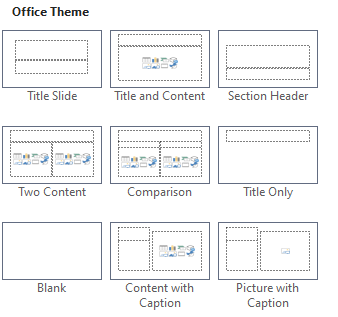
\includegraphics[width=0.5\linewidth]{imagens/tiposbasicosdopp}
    \caption{Slides básicos disponíveis no Power Point}
    \label{fig:tiposbasicosdopp}
\end{figure}

A Figura \ref{fig:tiposbasicosdopp}, copiada do \textit{Power Point} mostra esses seis tipos principais e mais alguns disponíveis para uma apresentação em branco, como o slide branco, e dois modelos com legenda. Já a Figura \ref{fig:vermelhao} mostra vários formatos de slides que eu criei no estilo que chamo de ``vermelhão'', mostrando uma gama de formatos que já usei.

\begin{figure}[hbt]
    \centering
    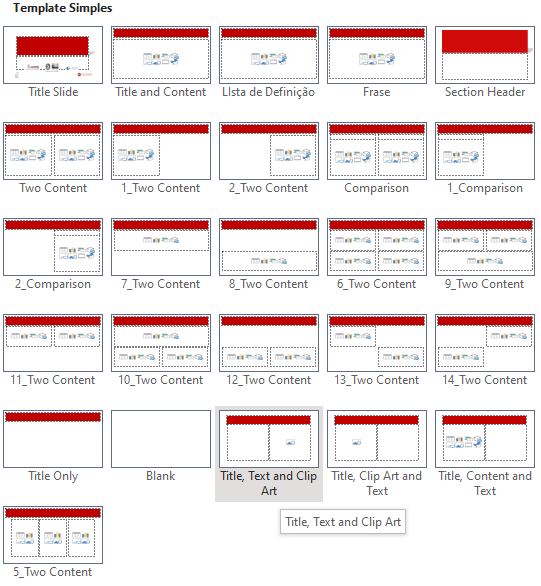
\includegraphics[width=0.5\linewidth]{imagens/vermelhao}
    \caption{Variantes de formatos de slide criados para um estilo, no Power Point.}
    \label{fig:vermelhao}
\end{figure}


Cada tipo de uso, como apresentação, aula, defesas ou exames, tem um estilo de slide mais adequado, de acordo com a necessidade de chamar atenção, e o grau de formalidade.

Em qualquer tipo de uso, porém, existem alguns objetos que devem aparecer nos slides, como a numeração e a identificação do autor e da instituição.

Os slides \textbf{devem ser numerados} e conter em cada slide o número total de slides, possivelmente no formato ``slide/total'', como em ``4/40''. Os números não podem ser pequenos, e eu favoreço números grandes, para que fique bem claro e possam, mesmo a distância, serem usados como referência. Esse número fica normalmente no rodapé (\textit{footer}) do slide.

Também é importante ter a identificação do autor. Normalmente ela inclui um e-mail ou um site.

Além disso, é interessante que, para a maioria dos usos, o estilo do slide esteja diretamente associado a uma instituição. Isso pode ser feito por meio da colocação do logo da instituição em uma posição clara.

No Power Point existem, por \textit{default}, três espaços no rodapé do slide (\textit{footer}). Um é reservado para o número. Os outros dois são possivelmente livres, sendo que um  sempre devemos usar identificar o autor. O terceiro espaço pode ser usado para o título da apresentação, o título do curso, o título do evento ou outra informação similar que se quer ressaltar.

A Figura \ref{fig:coppe} mostra um slide com todos esses elementos: o logo do PESC, o nome e e-mail do autor, o nome do curso, o número do slide em uma fonte grande e o número total de slides em uma fonte menor.



Devemos usar fontes ``limpas'', não rebuscadas, e \textbf{sem-serifa}\footnote{Serifas são as pontinhas que existem em algumas fontes. Elas estão bem visíveis no S da palavra ``slides'' desta seção.}, como Arial ou Calibri, e \textbf{corpos grandes}, 32 pts, por exemplo. Os slides das Figuras \ref{fig:coppe} e \ref{fig:teximag} seguem essa regra. Já o slide da figura \ref{fig:formulas} usa um tamanho menor para o corpo das fórmulas. Lembre que a banca, ao invés dos alunos, é mais velha e pode ter dificuldades de visão.





\subsection{Usando os logos corretos}

É \textbf{importantíssimo usar os logos corretos das instituições}. Para isso procure os logos originais e os manuais de marca.

No caso da UFRJ, houve um logo especial em 2020, para os 100 anos, e em 2021 o logo tradicional foi substituído por um logo moderno em azul. A variante vertical de uso preferencial é mostrada na Figura \ref{fig:logoufrj}. O PESC também tem um novo logo desde 2021, que é mostrado na Figura \ref{fig:logopesc}. Esse logo chegou a ser divulgado sem a referência a COPPE, e usar essa versão é errado.

\begin{figure}[hbt]
    \centering
    \subfloat[Logo vertical]{
    
\includegraphics[height=3cm]{imagens/UFRJ}\label{fig:logoufrjv}}
    \subfloat[Logo horizontal]{
    
\includegraphics[height=3cm]{imagens/UFRJH}\label{fig:logoufrjh}}
    \caption{Alguns dos logos novos da  UFRJ e partir de 2021. Existem versões com o nome completo que são de uso em contextos quando a UFRJ é menos conhecida.}
    \label{fig:logoufrj}
\end{figure}

\begin{figure}[hbt]
    \centering
    
\includegraphics[height=3cm]{imagens/logoPrincipal.eps}
    \caption{Logo novo do PESC.}
    \label{fig:logopesc}
\end{figure}



No GitHub que divulga este texto é possível baixar uma apresentação simples do PESC, feita em \textit{Power Point}, que usa os logos corretos\footnote{\url{https://github.com/xexeo/DicasSlidesAcademicos/tree/main/Slides}}.



A lista de logos que eu uso é:
\begin{itemize}
    \item UFRJ: \url{https://ufrj.br/comunicacao/manuais-e-modelos/marca-da-ufrj/}
    \item COPPE: \url{https://www.coppe.ufrj.br/pt-br/a-coppe/uso-da-marca}
    \item PESC:  \url{https://www.cos.ufrj.br/index.php/pt-BR/logo-pesc}
    \item IM: não fornece o logotipo na página, porém é possível copiar. A história da marca principal está em \url{https://sites.google.com/matematica.ufrj.br/mapcabral/outros/hist%C3%B3ria-do-logotipo-do-im}
    \item DCC: não fornece o logotipo na página, mas, de qualquer maneira, será transformado no IC, com novo logotipo
    \item POLI: \url{http://www.poli.ufrj.br/marcadapolitecnica.php}
    \item LUDES: \url{https://github.com/LUDES-PESC/Generico/tree/master/Logo%20Novo%20Vers%C3%B5es}
    \item LINE: \url{https://github.com/LINE-PESC/Generico/tree/master/Logomarca%20LINE}
\end{itemize}

No GitHub deste documento estão disponíveis algumas sugestões de slides.


\subsection{Nomeando os slides}

Todo slide deve ter um \textbf{título único}. Esse espaço já vem reservado nos estilos de \textit{Power Point}.

Algumas pessoas, erroneamente, usam um título de seção que se repete nessa posição e colocam o que seria o título do slide como uma caixa-de-texto, ou como primeiro item da lista de itens do slide. Essa prática faz com que a audiência se perca em relação a onde o apresentador está. O nome e o número do slides servem não só para identificá-los, mas também como posicionamento na sequência.

É possível criar um slide com o nome da seção, mas ele deve ser menor que o nome do slide. Usando o \texttt{beamer}, o formato de slides do \LaTeX, é possível colocar no topo do slide uma mini-agenda, onde o nome da seção tem uma ênfase. As Figuras \ref{fig:sistemas} e \ref{fig:meio} mostram  slides que têm todas as seções identificadas em seu cabeçalho, sendo que a seção atual está com ênfase.

Se for necessário ter dois slides com o mesmo nome, porque um é continuação do outro, numere os slides como foi feito na Figura \ref{fig:dados}, indicando também o total de slides dessa sequência com o mesmo nome, no formato ``(n/N)''.



\subsection{Slide de contato}

Como adicional, toda apresentação deve possuir um slide final que indica um contato. Hoje, todas as minhas aulas terminam com o slide da Figura \ref{fig:fim}. Isso pode ser usado sempre para falar algo como ``quem quiser me contatar para tirar dúvidas...''.

\begin{figure}[h]
    \centering
    
\includegraphics[width=\tam\linewidth,frame]{imagens/fim.png}
    \caption{Um slide de contato.}
    \label{fig:fim}
\end{figure}



